% Disable copyright notice in the bottom right corner of the document since this document 
%   is not the intellectual property of ASME
% Technically, ASME standards say all text must be in black when papers are submitted for 
%   publication, but this isn't going to be submitted so we can enable colorlinks to get 
%   links to show up as blue.
\documentclass[nofoot,pdf-a,balance,colorlinks,upint,subscriptcorrection,varvw,mathalfa=cal=boondoxo]{asmeconf}
\special{papersize=8.5in,11in}

% % enable use of multiple files 
% % https://www.overleaf.com/learn/latex/Multi-file_LaTeX_projects
% % \usepackage{subfiles}
% \usepackage[subpreambles=true]{standalone}
% \usepackage{import}

\usepackage{amsmath}
% prevent Bbbk from being overdefined by amsmath and newtxmath (from asmeconf.cls)
\let\Bbbk\relax
\usepackage{mathtools}
\usepackage{amssymb}
\usepackage{xfrac}
% \usepackage[margin=1.00in]{geometry}
% \usepackage{tabto}
\usepackage{tikz}
\usepackage{pgfplots}
\usepackage[thinc]{esdiff}
\usepackage{float}
\usepackage{graphicx}

% enable use of multiple files 
% https://www.overleaf.com/learn/latex/Multi-file_LaTeX_projects
\usepackage{subfiles}

% PDF meta data
\hypersetup{
	pdfauthor={Lucas S. Johnston, Brendan Moskalik},
    pdftitle={Solution for the Dynamics Piston Project},
	pdfkeywords={Dynamics, Piston, Pins, Reactive forces, Project},
	pdfsubject = {Solution for the Dynamics Piston Project},
}

% Default pgfplots settings to using the newest version and adding a grid
\pgfplotsset{
    compat = newest,
    grid = both,
}

\usetikzlibrary{arrows.meta}
\usetikzlibrary{positioning}
% for variables
\usetikzlibrary{math}
% for adding numbers to points
\usetikzlibrary{calc}

\begin{document}
    \ConfName{Proceedings of the Dynamics 2024 Local Mechanical Engineering Class and Exposition}
    \ConfDate{Spring, 2024} % update 
    \ConfCity{Spokane, WA}
    % let paper 0001 refer to our previous paper we submitted
    \PaperNo{ENSC2024-0002}

    \title{Piston Project}
    \SetAuthors{Lucas S. Johnston\affil{1}\JointFirstAuthor, Brendan Moskalik\affil{1}\JointFirstAuthor}
	\SetAffiliation{1}{Gonzaga University, Spokane, WA}

    \maketitle

    \begin{abstract}
        This paper is an analysis of the forces acting in pins within a crank-piston combination given a variety of cases. It analyzes the time-evolution of the system to derive an equation relating the forces in the pins to time in general, and applies specific conditions to create graphical representations of these forces for use in design. It is intended to be accompanied by a related MATLAB script \texttt{piston_script.m}, which is provided via a link to a git repository in the Appendix \ref{appendix:sources}.
    \end{abstract}

    \begin{nomenclature}
        \EntryHeading{Forces}
        \entry{$A$}{Shear force at A [N]}
        \entry{$P$}{Shear force at P [N]}

        \EntryHeading{Constant Parameters}
        \entry{$\omega$}{Angular velocity of the crank [rad s$^{-1}$]}
        \entry{$H$}{Offset distance between piston path and crank axis [m]}
        \entry{$L$}{Length of connecting rod [m]}
        \entry{$R$}{Distance from crank axis to point A [m]}
        \entry{$\theta_0$}{Initial angle of crank [rad]}
        \entry{$g$}{Gravitational acceleration [m s$^{-2}$]}\newline
       
        \EntryHeading{Time Evolution Parameters}
        \entry{$t$}{Time [s]}
        \entry{$\omega_{\textrm{AP}}$}{Angular velocity of the rod AP [rad s$^{-1}$]}
        \entry{$\alpha_{\textrm{AP}}$}{Angular acceleration of the rod AP [rad s$^{-2}$]}
        \entry{$m$}{Mass [kg]}
        \entry{$\vec{r}$}{Position [m]}
        \entry{$\vec{v}$}{Translational velocity [m s$^{-1}$]}
        \entry{$\vec{a}$}{Translational acceleration [m s$^{-2}$]}
        \entry{$\theta$}{Angle of crank with horizontal [rad]}\newline

        % TODO -- find a way to incorporate subscripts that 
        \EntryHeading{Superscripts and subscripts}
        \entry{x}{Horizontal component}
        \entry{y}{Vertical component}
        \entry{O}{Point O value}
        \entry{A}{Point A value}
        \entry{P}{Point P value}
        \entry{G}{Connecting rod center of gravity value}
        \entry{$\,\sfrac{\textrm{b}}{\textrm{a}}$}{Value from a to b, where a and b are any points}
        \entry{p}{Piston value}
        \entry{c}{Connecting rod AP value}
        \entry{$AP$}{Connecting rod AP value}
        
    \end{nomenclature}

    \section{Problem Statement}

    We are given a slider-crank piston setup explicitly parameterized by $L$, $R$, $H$, $\omega$, and $\theta$. With the exception of $\theta$, these parameters are all constant with respect to time. Information on these constant parameters can be found in Appendix \ref{appendix:cases}. The mass of the connecting rod and the piston ($m_{\textrm{c}}$ and $m_{\textrm{p}}$ respectively) are known, as is $R$. The rod is a cylinder with uniformly distributed mass per unit length.
    
    \begin{figure}[H]
        \centering
    	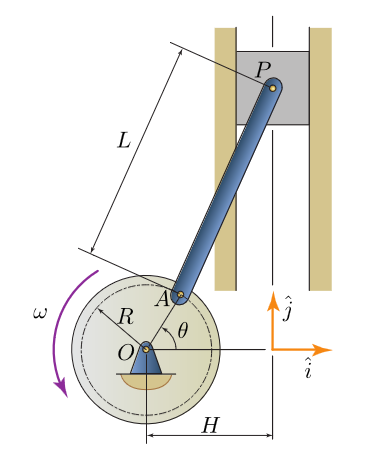
\includegraphics[scale=0.45]{problem_diagram.png}
    	\caption{Offset slider-crank piston, as given}\label{fig:diagram}
    \end{figure}

    \begin{table}[H]
        \caption[Table]{Case-Independent Known Values}\label{tab:given}
        \centering{
            \begin{tabular}{llr}
            \toprule
            Value & Value  & Units \\
            \midrule
                $R$ & 0.075 & m \\
                $m_{\textrm{c}}$ & 0.3 & kg \\
                $m_{\textrm{p}}$ & 0.4 & kg \\
            \bottomrule
            \end{tabular}
        }
    \end{table}

    The crank rotates about a fixed axis O. The piston is constrained to move up and down in the direction of the $\hat{\jmath}$ elementary vector as drawn. All motion is constrained to the plane spanned by $\hat{\imath}$ and $\hat{\jmath}$.


    \section{Solution Derivation}

    Let's solve the generic solution, and then apply specific cases to it once we've obtained useful formulas. We are interested in how the system evolves as $\theta$ changes. The rate of change of $\theta$, $\omega$ is given as a known constant. Therefore, we can parameterize $\theta$ as follows.
    \begin{equation} 
        \theta = \omega t + \theta_0
    \end{equation}
    Here, $\omega$ must be in radians per second (and therefore has to be converted from the as-given speeds given in rpm). $\theta_0$ refers to the initial condition of $\theta$ when $t = 0$ seconds.

    We are interested in finding the angular and translational acceleration of G, the center of gravity of the connecting rod for use in solving reactive forces at the pins A and B.


    This allows us to construct the position vector of A. Let the origin be set at fixed point O.

    \begin{equation} 
        \vec{r}_{\textrm{A}} = R\cdot\left(\cos{\left(\theta\right)}\hat{\imath} + \sin{\left(\theta\right)}\hat{\jmath}\right)
    \end{equation}


    The point A is constained to circular motion with a constant radius about the crank with a constant angular velocity.

    \begin{equation} 
        \vec{v}_{\textrm{A}} = \vec{0} + \omega\hat{k}\times\vec{r}_{\textrm{A}} = \omega\cdot\vec{r}_{\textrm{A}}
    \end{equation}


    Here $\hat{k}$ is a unit vector that, together with $\hat{\imath}$ and $\hat{\jmath}$, spans $\mathbb{R}^3$. This allows the cross product to be defined. $\hat{k}$ is normal to both $\hat{\imath}$ and $\hat{\jmath}$, and form the basis for a Cartesian representation of vectors in three-space in a Right Handed coordinate system. The angular velocity $\omega$ is given to us in a direction pointing in the $+\hat{k}$ direction.

    Let's now find the angular velocity of the rod to determine its acceleration. Since the rod has a constant length $L$, we can apply the following.

    \begin{equation} 
        % \, is a small space
        \vec{v}_{\,\textrm{P}} = \vec{v}_{\textrm{A}} + \omega_{\textrm{AP}}\hat{k}\times \vec{r}_{\,\sfrac{\textrm{P}}{\textrm{A}}}
    \end{equation}

    Note that $\alpha_{\textrm{AP}}$ is defined that a positive quantity means counter-clockwise rotation. To find $\vec{r}_{\,\sfrac{\textrm{P}}{\textrm{A}}}$, we can build P's position from O.

    \begin{equation}
        \vec{r}_{\,\sfrac{\textrm{P}}{\textrm{A}}} + \vec{r}_{\textrm{A}} = \vec{r}_{\,\textrm{P}}
    \end{equation}
    \begin{equation}
        \hat{\imath}\cdot \left(\vec{r}_{\,\sfrac{\textrm{P}}{\textrm{A}}} + \vec{r}_{\textrm{A}}\right) = \hat{\imath} \cdot \left(\vec{r}_{\,\textrm{P}}\right)
    \end{equation}
    \begin{equation}
        \hat{\imath}\cdot \vec{r}_{\,\sfrac{\textrm{P}}{\textrm{A}}} = \hat{\imath} \cdot \vec{r}_{\,\textrm{P}} - \hat{\imath} \cdot\vec{r}_{\textrm{A}} 
    \end{equation}
    \begin{equation}
        \hat{\imath}\cdot \vec{r}_{\,\sfrac{\textrm{P}}{\textrm{A}}} = H - R\cdot\cos{\left(\theta\right)}
    \end{equation}

    Applying the constraint that the distance from point A to point P is $L$, we get the following.

    \begin{equation} 
        L^2 = \left(\vec{r}_{\,\sfrac{\textrm{P}}{\textrm{A}}} \cdot\hat{\imath} \right)^2+ \left(\vec{r}_{\,\sfrac{\textrm{P}}{\textrm{A}}} \cdot\hat{\jmath}\right)^2
    \end{equation}

    Since the vertical component of $\vec{r}_{\,\sfrac{\textrm{P}}{\textrm{A}}}$ is positive as drawn in Fig \ref{fig:diagram}, we use the positive root.
    \begin{equation} 
        \vec{r}_{\,\sfrac{\textrm{P}}{\textrm{A}}} \cdot\hat{\jmath} = \sqrt{L^2 - \left(\vec{r}_{\,\sfrac{\textrm{P}}{\textrm{A}}} \cdot\hat{\imath} \right)^2}
    \end{equation}
    \begin{equation} 
        \vec{r}_{\,\sfrac{\textrm{P}}{\textrm{A}}} \cdot\hat{\jmath} = \sqrt{L^2 - \left(H - R\cdot\cos{\left(\theta\right)}\right)^2}
    \end{equation}

    $\vec{r}_{\,\sfrac{\textrm{P}}{\textrm{A}}}$ is now well-defined.

    \begin{equation} 
        \vec{r}_{\,\sfrac{\textrm{P}}{\textrm{A}}} = \left(H - R\cdot\cos{\left(\theta\right)}\right)\hat{\imath} + \left(\sqrt{L^2 - \left(H - R\cdot\cos{\left(\theta\right)}\right)^2}\right)\hat{\jmath}
    \end{equation}

    To simplify resultant expressions, we will introduce intermediate variables $h$ and $l$ as follows. The full version of expressions shown below expressed purely in terms of constant parameters and time may be references in Appendix \ref{appendix:definitions}.

    \begin{equation} 
        h = \vec{r}_{\,\sfrac{\textrm{P}}{\textrm{A}}} \cdot \hat{\imath}
    \end{equation}
    \begin{equation} 
        l = \vec{r}_{\,\sfrac{\textrm{P}}{\textrm{A}}} \cdot \hat{\jmath}
    \end{equation}

    
    We can now use the fact that $\vec{v}_{\,\textrm{P}}$ is constrained to purely vertical movement. Let $v_{\,\textrm{P}} = \vec{v}_{\,\textrm{P}} \cdot \hat{\jmath}$. 

    \begin{equation}\label{eq:velocity_system}
        v_{\,\textrm{P}}\hat{\jmath} = \vec{v}_{\textrm{A}} + \omega_{\textrm{AP}}\hat{k}\times \vec{r}_{\,\sfrac{\textrm{P}}{\textrm{A}}}
    \end{equation}

    Every variable in the above expression is a `known' quantity expressible purely in terms of constant parameters and time, with the exception of $v_{\,\textrm{P}}$ and $\omega_{\textrm{AP}}$. These scalar quantities are, in essence, two degrees of freedom now being constrained within a vector equation. This vector equation can be broken into two linearly dependent equations, which suggest $v_{\,\textrm{P}}$ and $\omega_{\textrm{AP}}$ are both well-defined. Linear algebra is now sufficient to prove the following\footnote{The overall process consists of re-organizing the system of equations to put linear combinations of what we hope to solve on the right hand side, and everything else on the left hand side. Factoring out a two-by-two matrix over the reals suggests taking a matrix inverse to solve for our two unknowns in terms of what we already know. This algebra is solved within the accompanying script \texttt{piston_script.m}, which shares the same nomenclature as defined within this document. It may be helpful to reference this script to understand the results.}.

    \subfile{autogen_vel}

    What we are truly interested in are the accelerations throughout the system. Let's begin solving for these. Since point A rotates about O with a constant angular veloctity constrained to uniform circular motion, its acceleration is described as follows.


    \begin{equation}
        \vec{a}_{\textrm{A}} = - \omega^2\cdot\vec{r}_{\textrm{A}}
    \end{equation}

    The acceleration of the piston can be described as follows.


    \begin{equation}
        \vec{a}_{\textrm{p}} = \vec{a}_{\textrm{A}} + \alpha_{\textrm{AP}}\hat{k} \times \vec{r}_{\,\sfrac{\textrm{P}}{\textrm{A}}} + \omega_{\textrm{AP}}\hat{k}\times \left(\omega_{\textrm{AP}}\hat{k}\times \vec{r}_{\,\sfrac{\textrm{P}}{\textrm{A}}}\right)
    \end{equation}

    Note that $\alpha_{\textrm{AP}}$ is defined such that a positive value denotes counter-clockwise acceleration. Since all motion in this system is confined to the plane, the equation can be reduced.

    \begin{equation}\label{eq:piston_accel}
        \vec{a}_{\textrm{p}} = \vec{a}_{\textrm{A}} + \alpha_{\textrm{AP}}\hat{k} \times \vec{r}_{\,\sfrac{\textrm{P}}{\textrm{A}}} - \omega_{\textrm{AP}}^2 \vec{r}_{\,\sfrac{\textrm{P}}{\textrm{A}}}
    \end{equation}

    The piston's motion being constrained to the $\hat{\jmath}$ direction also means its acceleration is constrained to that direction. Let $a_{\textrm{p}} = \vec{a}_{\textrm{p}}\cdot\hat{\jmath}$.

    \begin{equation}
         a_{\textrm{p}}\hat{\jmath}= \vec{a}_{\textrm{A}} + \alpha_{\textrm{AP}}\hat{k} \times \vec{r}_{\,\sfrac{\textrm{P}}{\textrm{A}}} - \omega_{\textrm{AP}}^2 \vec{r}_{\,\sfrac{\textrm{P}}{\textrm{A}}}
    \end{equation}

    With the exception of $a_{\textrm{p}}$ and $\alpha_{\textrm{AP}}$, every term in this expression has already been explicitly described in terms of the system's constant parameters and $t$. These two scalar quantities can be considered two `unknowns' in two systems of equations if one looks at the horizontal and vertical terms of this vector equation as two seperate scalar equation. Using similiar linear algebra techniques as applied to Eq. \eqref{eq:velocity_system}, we can demonstrate the following.

    \subfile{autogen_acc}

    We are told the connecting rod AP is a uniform cylinder. This means its center of gravity lies halfway along its length.

    \begin{equation}
        \vec{r}_{\,\sfrac{\textrm{G}}{\textrm{A}}} = \frac{1}{2}\cdot \vec{r}_{\,\sfrac{\textrm{P}}{\textrm{A}}}
    \end{equation}

    The translational acceleration of G can be found similiarly to Eq. \eqref{eq:piston_accel}. Recall that rigid bodies have one angular acceleration and velocity throughout.

    \begin{equation}
        \vec{a}_{\textrm{G}} = \vec{a}_{\textrm{A}} + \alpha_{\textrm{AP}}\hat{k} \times \vec{r}_{\,\sfrac{\textrm{G}}{\textrm{A}}} - \omega_{\textrm{AP}}^2 \vec{r}_{\,\sfrac{\textrm{G}}{\textrm{A}}}
    \end{equation}

    We now have enough acceleration information to begin considering free body diagrams. There are two bodies of interest here, the connecting rod and the piston.



    % defines variables within tikz environments 
    \tikzmath{
        \forceoffset = 0.10;
    }

    \begin{figure}[H]
        \centering
        \begin{tikzpicture}
            % Rod
            \coordinate (A) at (-1.5/1.75,-3/1.75);
            \coordinate (P) at (1.5/1.75,3/1.75);
            \draw (A)node[left]{A} -- (P)node[left]{P};
            % Center of Gravity
            \filldraw[fill=white](0,0) circle(0.1);
            \draw [fill=black] (0,0) -- ++(0.1,0) arc(0:90:0.1) -- cycle;
            \draw [fill=black] (0,0) -- ++(-0.1,0) arc(180:270:0.1) -- cycle;
            \node [right = 2.0pt](0,0) {G};


            % Forces
            \draw [-Stealth, violet] (0,-0.1 - \forceoffset) -- (0,-1) node[below] {$m_{\textrm{c}} g$};
            \draw [-Stealth, violet] ($ (A) + (\forceoffset,0)$) -- ($(A) + (1 + \forceoffset,0)$) node[below] {$A_x$};
            \draw [-Stealth, violet] ($ (A) + (0,\forceoffset)$) -- ($(A) + (0,1 + \forceoffset)$) node[above] {$A_y$};
            \draw [-Stealth, violet] ($ (P) + (\forceoffset,0)$) -- ($(P) + (1 + \forceoffset,0)$) node[below] {$P_x$};
            \draw [-Stealth, violet] ($ (P) + (0,\forceoffset)$) -- ($(P) + (0,1 + \forceoffset)$) node[above] {$P_y$};

            % coordinate system
            \coordinate (a) at (4,0);
            \coordinate (b) at (5,0);
            \coordinate (c) at (4,1);
            \draw (a) -- (b)node[right]{$\hat{\imath}$};
            \draw (a) -- (c)node[above]{$\hat{\jmath}$};
            \draw [-Stealth] ($(a) + (0.1,0.1) + (0.55cm,0)$) arc(0:90:0.55cm) node[midway,above] {$\hat{k}$};

        \end{tikzpicture}
        \caption{Free Body Diagram of the Connecting Rod}
    \end{figure}
    \begin{figure}[H]
        \centering
        \begin{tikzpicture}
            % Rectangle
            \coordinate (A) at (-1.5,-1);
            \coordinate (B) at (-1.5,1);
            \coordinate (C) at (1.5,1);
            \coordinate (D) at (1.5,-1);
            \draw (A) -- (B);
            \draw (B) -- (C);
            \draw (C) -- (D);
            \draw (D) -- (A);
            % Center of Gravity
            \filldraw[fill=white](0,0) circle(0.1);
            \draw [fill=black] (0,0) -- ++(0.1,0) arc(0:90:0.1) -- cycle;
            \draw [fill=black] (0,0) -- ++(-0.1,0) arc(180:270:0.1) -- cycle;
            \node [right = 2.0pt](0,0) {P};


            % Forces
            \draw [-Stealth, violet] (0,-0.1 - \forceoffset) -- (0,-1.5) node[right] {$P_y$};
            \draw [-Stealth, violet] (-0.1 - \forceoffset,0) -- (-1.75,0) node[left] {$P_x$};
            \draw [-Stealth, violet] (0,-1.5-\forceoffset) -- (0,-2) node[below] {$m_{\textrm{p}} g$};
            \draw [Stealth-Stealth, violet] (1.5+\forceoffset,0) -- (2.5,0) node[right] {$N$};

            % coordinate system
            \coordinate (a) at (4,0);
            \coordinate (b) at (5,0);
            \coordinate (c) at (4,1);
            \draw (a) -- (b)node[right]{$\hat{\imath}$};
            \draw (a) -- (c)node[above]{$\hat{\jmath}$};

        \end{tikzpicture}
        \caption{Free Body Diagram of the Piston}
    \end{figure}

    Here, $N$ represents the normal force on the piston block exerted by its track simplified from a distributed force to a single point force. Let's sum forces on the piston block in the $\hat{\jmath}$ direction. Note that point P is coincident with the piston block's center of gravity/mass.

    \begin{equation}
        \hat{\jmath}\cdot \sum{\vec{F}} = \hat{\jmath}\cdot m_{\,\textrm{P}}\vec{a}_{\,\textrm{P}}
    \end{equation}
    \begin{equation}
        -P_y - m_{\,\textrm{P}}g = m_{\,\textrm{P}}a_{\,\textrm{P}}
    \end{equation}

    From this relation, we can derive our first pin force.

    \begin{equation}
        P_y = -m_{\,\textrm{P}}a_{\,\textrm{P}} -  m_{\,\textrm{P}}g
    \end{equation}
    \begin{equation}
        P_y = -m_{\,\textrm{P}}\left(a_{\,\textrm{P}} +  g\right)
    \end{equation}

    \subfile{autogen_P_y}

    Now that we know the values of one of our forces, summing forces and moments about the rod AP is sufficient to fully define the remaining forces\footnote{It is easy to be mislead by summing forces across the rod AP and moments about point A and point P that we \textit{only} need to use the free body diagram for the rod. However, these relations alone are not well-posed, and need one force to be specified beforehand to yield useful results.}.

    \begin{equation}
        \sum{\vec{F}} = m_{\,\textrm{AP}}\vec{a}_{\,\textrm{G}}
    \end{equation}
    \begin{equation}\label{sum:forces}
        \begin{bmatrix}
            A_x + P_x \\
            A_y + P_y - m_{\,\textrm{c}}g \\
        \end{bmatrix} = 
        \begin{bmatrix}
            m_{\,\textrm{c}}\vec{a}_{\,\textrm{G}} \cdot \hat{\imath} \\
            m_{\,\textrm{c}}\vec{a}_{\,\textrm{G}} \cdot \hat{\jmath} \\
        \end{bmatrix}
    \end{equation}

    Since we already know the right hand side of this equation in terms of our desired parameters, and we've just solved for $P_y$, we know enough to solve for $A_y$.

    \begin{equation} 
        A_y + P_y - m_{\,\textrm{c}}g  = m_{\,\textrm{c}}\vec{a}_{\,\textrm{G}} \cdot \hat{\jmath}
    \end{equation}
    
    \begin{equation} 
        A_y = m_{\,\textrm{c}}\vec{a}_{\,\textrm{G}} \cdot \hat{\jmath} +  m_{\,\textrm{c}}g - P_y
    \end{equation}

    \subfile{autogen_A_y}

    While it is possible to sum moments anywhere, it somewhat simplifies things if we sum forces about A or P. Let's chose point A.

    \begin{equation}
        \hat{k}\cdot\sum{\vec{M}_{\textrm{A}}} = I_{\textrm{A}}\alpha_{\textrm{AP}}
    \end{equation}

    Firstly, we need to construct the mass moment of inertia of a thin rod rotating in the $\hat{k}$ direction.


    \begin{equation} 
        I_{\textrm{A}} = I_{\textrm{G}} + m_{\,\textrm{c}}{\left(\frac{L}{2}\right)}^2
    \end{equation}

    \begin{equation} 
        I_{\textrm{G}} = \frac{1}{12}m_{\,\textrm{c}}L^2
    \end{equation}

    Recalling the definition of a moment, we get the following.

    \begin{equation}
        \hat{k}\cdot\left(\vec{r}_{\,\sfrac{\textrm{P}}{\textrm{A}}} \times \left(P_x \hat{\imath} + P_y \hat{\jmath}\right) + \vec{r}_{\,\sfrac{\textrm{G}}{\textrm{A}}}\times\left(-m_{\,\textrm{c}}g\hat{\jmath}\right)\right)  = I_{\textrm{A}}\alpha_{\textrm{AP}}
    \end{equation}

    Knowing $P_y$ means the above expression fully defines $P_x$.

    \subfile{autogen_P_x}

    Going back to Eq. \eqref{sum:forces}, we can solve for the final missing reactice force, $A_x$.

    \begin{equation}
            A_x + P_x = m_{\,\textrm{c}}\vec{a}_{\,\textrm{G}} \cdot \hat{\imath}
    \end{equation}

    \begin{equation}
            A_x = m_{\,\textrm{c}}\vec{a}_{\,\textrm{G}} \cdot \hat{\imath} -  P_x 
    \end{equation}

    \subfile{autogen_A_x}


    $A$ represents the magnitude of the forces on the pin at A and $P$ represents the magnitude of the forces on the pin at P.  Using the property of the magnitude of vectors, we arrive at the following.
    \begin{equation}
        A = \sqrt{A_{\textrm{x}}^2 + A_{\textrm{y}}^2}
    \end{equation}
    \begin{equation}
        P = \sqrt{P_{\textrm{x}}^2 + P_{\textrm{y}^2}}
    \end{equation}

    \subfile{autogen_AandP}
    


computing the maximum values of the forces in the pins gives us
\begin{table}[H]
        \caption[Table]{Max forces at A - Case1}\label{tab:aForce1}
        \centering{
            \begin{tabular}{llr}
            \toprule
           $\omega$ (rev/m)  & $\theta$ (rad) & max force (N) \\
            \midrule
                1000& 1.5708 & 881.49 \\
	2200 & 1.5708&4251.3 \\
	5000 &1.5708&21943 \\
            \bottomrule
            \end{tabular}
        }
    \end{table}
\begin{table}[H]
        \caption[Table]{Max forces at A - Case2}\label{tab:aForce2}
        \centering{
            \begin{tabular}{llr}
            \toprule
           $\omega$ (rev/m)   & $\theta$ (rad) & max force (N) \\
            \midrule
                1000 &1.5708 & 755.89 \\
	2200&1.5708&3643.3\\
	5000&1.5708&18802\\
            \bottomrule
            \end{tabular}
        }
    \end{table}
\begin{table}[H]
        \caption[Table]{Max forces at A - Case3}\label{tab:aForce3}
        \centering{
            \begin{tabular}{llr}
            \toprule
           $\omega$ (rev/m) & $\theta$ (rad) & max force (N) \\
            \midrule
                1000 &1.2566&762.04 \\
	2200&3.4558&3699\\
	5000&3.4558&19132\\
            \bottomrule
            \end{tabular}
        }
    \end{table}


\begin{table}[H]
        \caption[Table]{Max forces at P - Case 1}\label{tab:pForce1}
        \centering{
            \begin{tabular}{llr}
            \toprule
          $\omega$ (rev/m)  & $\theta$ (rad) & max force (N) \\
            \midrule
                1000 & 1.5708 &552.43 \\
	2200 &1.5708&2658.7 \\
	5000&1.5708&13717 \\
            \bottomrule
            \end{tabular}
        }
    \end{table}
\begin{table}[H]
        \caption[Table]{Max forces at P - Case 2}\label{tab:pForce2}
        \centering{
            \begin{tabular}{llr}
            \toprule
          $ \omega$ (rev/m)& $\theta$ (rad) & max force (N) \\
            \midrule
                1000&1.5708 & 463.4 \\
	2200&1.5708&2227.6\\
	5000&1.5708&11489\\
            \bottomrule
            \end{tabular}
        }
    \end{table}
\begin{table}[H]
        \caption[Table]{Max forces at P - Case 3}\label{tab:pForce3}
        \centering{
            \begin{tabular}{llr}
            \toprule
           $\omega$ (rev/m)  & $\theta$ (rad) & max force (N) \\
            \midrule
                1000&3.4558&558.45 \\
	2200&3.4558&2726.3\\
	5000&3.4558&14108\\
            \bottomrule
            \end{tabular}
        }
    \end{table}

	\section{Discussion of results}
	One very clear verification we can do is check that they cycle is actually repeatable. This means that the value and slope at the end of the cylce and begining of the cylce should be equivalent. This is something you can easily see in our graphs holds true, which is good. 


	As can be seen in our graphs increasing $\omega$ to higher speeds the forces felt in the pins are higher. This is true across all the cases. it also makes sense as higher values of $\omega$ should reult in higher accelerations. Higher accelerations we know will result in higer forces on the pins.
    
    To further check our results, the bulk of the heavy lifting in terms of algebra was done via a MATLAB script, where position vectors were also created for each of the positions we solved the velocity and acceleration of as functions of time. Because of this, we can check our results for the velocity and accleration at that point versus a `naïve' time derivative approach by comparring for equality. This was done via a custom method which first checked if the expressions were written in the same form, if they could be proved equivalent, and finally, for more complicated expressions, if their numerical output for a random set of inputs are within a floating point comparison tolerance of each other. This method was used throughout the code, and would throw an error if a discrepancy emerged that suggested we'd made an algebra or sign error throughout our process.


	Case 2 tended to have the smallest forces of the three cases. This indicated that $\sfrac{L}{R}$ and $\sfrac{H}{R}$ have opposite effects on the system. As in case 1, Low values for both of these resulted in a higher max force at A, wheras in case 3, we have a more even value of the max forces spread between A and P.

	The next steps for this project to make it more realistic would start with modeling the force on the piston from the gas. It would not be to complicated to get this from the ideal gas laws, and would make the model much more useful. This allows to actually see how the engine actually would perform. In the project we just testing a few values for $\omega$ 4 but we have no idea if those are correct or useful running speeds for the engine. A force pushing the piston down would be able to give us more accurate values for this. The step after that would be to add a load to the output, allowing the calulation to be even more accurate for this usecase. An engine also does not have constant power output, so if we model the piston force we can incorperate that into our model and account for the fact that in a four stroke engine, only 1 out of every 4 piston moves actually is pushing down on it. Both the exaust and intake are almost free spinning other than friction, but there also would be the compression stage to account for. Adding the force to the piston would allow us to model this loss in power as its a force working against the engines motion. Then if we have mutiple cylinders we can see how much losses we need for the engine to keep running. 


    \appendix
    \section{Cases}\label{appendix:cases}
	  \begin{table}[H]
        \caption[Table]{Cases to consider (Given)}\label{tab:givenCases}
        \centering{
            \begin{tabular}{llr}
            \toprule
            Case & L/R  & H/R \\
            \midrule
                1 & \sfrac{3}{2} & 0 \\
                2 & \sfrac{8}{3} & \sfrac{1}{3} \\
                3 & 4 & \sfrac{5}{3} \\
            \bottomrule
            \end{tabular}
        }
    \end{table}

	Since we know the radius of all these cases to be 0.075 m we can compute values for L and H. Plugging those in:
\begin{table}[H]
        \caption[Table]{Cases to consider (Absolute)}\label{tab:absCases}
        \centering{
            \begin{tabular}{llr}
            \toprule
            Case & L (m)  & H (m) \\
            \midrule
                1 & 0.1124 & 0 \\
                2 & 0.2 & 0.025 \\
                3 & 0.3 & 0.125 \\
            \bottomrule
            \end{tabular}
        }
    \end{table}


    \subfile{autogen_fn_def}

    \subfile{autogen_graphs}

    \section{Sources}\label{appendix:sources} 

    This document was written with \LaTeX\ and is designed to be compilled by a valid \LaTeX\ engine such as \texttt{pdfTeX}. The git repository used to generate this document can be found online on GitHub at \href{https://github.com/A-Person7/dynamics_piston_project}{https://github.com/A-Person7/dynamics_piston_project}. MATLAB's symbolic toolbox was used to solve a lot of the linear algebra shown throughout this document, as well as to generate equations. These were implemented in the MATLAB script file \texttt{piston_script.m}. Compilation instructions for the final document are provided in the plain-text file \texttt{README}.


    \end{document}
